\begin{table}[p]
   \centering
   \footnotesize
   \renewcommand{\arraystretch}{1.15}
   \begin{tabular}{@{}>{\centering\arraybackslash}m{0.3033\textwidth}>{\centering\arraybackslash}m{0.3033\textwidth}>{\centering\arraybackslash}m{0.3033\textwidth}@{}}
      \hline
      \multicolumn{3}{@{}c@{}}{%
         \begin{tabular}{@{}>{\centering\arraybackslash}m{\dimexpr0.455\textwidth+\tabcolsep\relax}>{\centering\arraybackslash}m{\dimexpr0.455\textwidth+\tabcolsep\relax}@{}}
            $K_{3,5}$ & Matriz de adyacencia \\
            \hline
            \noalign{\vspace{6pt}}
            \rule{0pt}{0pt}$\vcenter{\hbox{\resizebox{0.3\textwidth}{!}{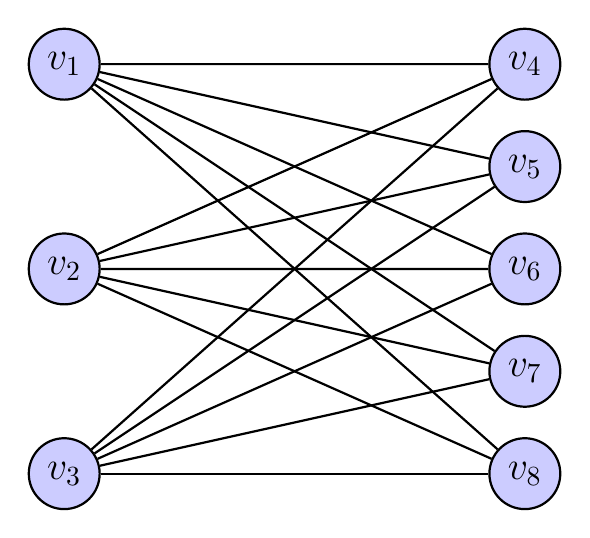
\begin{tikzpicture}[
  scale=1.3,
  vnode/.style={circle, fill=blue!20, draw=black, thick, minimum size=9mm, inner sep=0pt, font=\Large}
]
  % Partición izquierda
  \node[vnode] (v1) at (0, 4) {$v_1$};
  \node[vnode] (v2) at (0, 2) {$v_2$};
  \node[vnode] (v3) at (0, 0) {$v_3$};

  % Partición derecha
  \foreach \j in {4,...,8} {
    \node[vnode] (v\j) at (4.5, {8-\j}) {$v_{\j}$};
  }

  % Aristas: cada vértice de la izquierda con cada vértice de la derecha
  \foreach \i in {1,2,3} {
    \foreach \j in {4,...,8} {
      \draw[thick] (v\i) -- (v\j);
    }
  }
\end{tikzpicture}
}}}$
            &
            $\vcenter{\hbox{$\displaystyle \begin{pmatrix}
         0 & 0 & 0 & 1 & 1 & 1 & 1 & 1 \\
         0 & 0 & 0 & 1 & 1 & 1 & 1 & 1 \\
         0 & 0 & 0 & 1 & 1 & 1 & 1 & 1 \\
         1 & 1 & 1 & 0 & 0 & 0 & 0 & 0 \\
         1 & 1 & 1 & 0 & 0 & 0 & 0 & 0 \\
         1 & 1 & 1 & 0 & 0 & 0 & 0 & 0 \\
         1 & 1 & 1 & 0 & 0 & 0 & 0 & 0 \\
         1 & 1 & 1 & 0 & 0 & 0 & 0 & 0
      \end{pmatrix}$}}$ \\
            \noalign{\vspace{6pt}}
         \end{tabular}%
      } \\
      \hline
      \multicolumn{3}{c}{\textbf{Topología de adyacencia}} \\
      \hline
      Abiertos subbásicos & Vecindades mínimas & Topología \\
      \hline
         ${A_{v_1}=\{v_4,v_5,v_6,v_7,v_8\}}$\par
         ${A_{v_2}=\{v_4,v_5,v_6,v_7,v_8\}}$\par
         ${A_{v_3}=\{v_4,v_5,v_6,v_7,v_8\}}$\par
         ${A_{v_4}=\{v_1,v_2,v_3\}}$\par
         ${A_{v_5}=\{v_1,v_2,v_3\}}$\par
         ${A_{v_6}=\{v_1,v_2,v_3\}}$\par
         ${A_{v_7}=\{v_1,v_2,v_3\}}$\par
         ${A_{v_8}=\{v_1,v_2,v_3\}}$
      &
         ${U_{v_1}=\{v_1,v_2,v_3\}}$\par
         ${U_{v_2}=\{v_1,v_2,v_3\}}$\par
         ${U_{v_3}=\{v_1,v_2,v_3\}}$\par
         ${U_{v_4}=\{v_4,v_5,v_6,v_7,v_8\}}$\par
         ${U_{v_5}=\{v_4,v_5,v_6,v_7,v_8\}}$\par
         ${U_{v_6}=\{v_4,v_5,v_6,v_7,v_8\}}$\par
         ${U_{v_7}=\{v_4,v_5,v_6,v_7,v_8\}}$\par
         ${U_{v_8}=\{v_4,v_5,v_6,v_7,v_8\}}$
      &
         $\{\emptyset,$ $\{v_1,v_2,v_3\},$ $\{v_4,v_5,v_6,v_7,v_8\},$ $\{v_1,\allowbreak v_2,\allowbreak v_3,\allowbreak v_4,\allowbreak v_5,\allowbreak v_6,\allowbreak v_7,\allowbreak v_8\}\}$ \\[6pt]
      \hline
      \multicolumn{3}{c}{\textbf{Topología de incidencia}} \\
      \hline
      Abiertos subbásicos & Vecindades mínimas & Topología \\
      \hline
         \vspace{3pt}\begin{tabular}{@{}l@{\hspace{1.2em}}l@{}}
            ${e_{1}=\{v_1,v_4\}}$ & ${e_{9}=\{v_2,v_7\}}$ \\
            ${e_{2}=\{v_1,v_5\}}$ & ${e_{10}=\{v_2,v_8\}}$ \\
            ${e_{3}=\{v_1,v_6\}}$ & ${e_{11}=\{v_3,v_4\}}$ \\
            ${e_{4}=\{v_1,v_7\}}$ & ${e_{12}=\{v_3,v_5\}}$ \\
            ${e_{5}=\{v_1,v_8\}}$ & ${e_{13}=\{v_3,v_6\}}$ \\
            ${e_{6}=\{v_2,v_4\}}$ & ${e_{14}=\{v_3,v_7\}}$ \\
            ${e_{7}=\{v_2,v_5\}}$ & ${e_{15}=\{v_3,v_8\}}$ \\
            ${e_{8}=\{v_2,v_6\}}$ &  \\
         \end{tabular}\vspace{3pt}
      &
         \vspace{3pt}\begin{tabular}{@{}l@{\hspace{1.2em}}l@{}}
            ${U_{v_1}=\{v_1\}}$ & ${U_{v_5}=\{v_5\}}$ \\
            ${U_{v_2}=\{v_2\}}$ & ${U_{v_6}=\{v_6\}}$ \\
            ${U_{v_3}=\{v_3\}}$ & ${U_{v_7}=\{v_7\}}$ \\
            ${U_{v_4}=\{v_4\}}$ & ${U_{v_8}=\{v_8\}}$ \\
         \end{tabular}\vspace{3pt}
      &
         $\wp\left(V\left(K_{3,5}\right)\right)$ \\[6pt]
      \hline
   \end{tabular}
   \caption{Topologías de adyacencia e incidencia de $K_{3,5}$}
   \label{tab:topologias_K_35}
\end{table}
